\documentclass[a4paper]{article}

\def\npart {Mathematical Modeling Foundations}
\def\nterm {Matrix, dynamics, geometry}
\def\nyear {2026}
\def\nlecturer {MIT 6.S087/18.03/18.031/18.335/18.337/6.441/6.435; MBAM/QSP}
\def\ncourse {From Matrix Tricks to MBAM}
\def\ncoursehead {Matrix to MBAM}
\def\nauthor {NanFangHong}

\RequirePackage{etex}
\makeatletter
\ifx \npart \undefined
  \def\npart{PK/PD Notes}
\fi
\ifx \nterm \undefined
  \def\nterm{Reading notes}
\fi
\ifx \nyear \undefined
  \def\nyear{\the\year}
\fi
\ifx \nlecturer \undefined
  \def\nlecturer{the source literature}
\fi
\ifx \nauthor \undefined
  \def\nauthor{NanFangHong}
\fi
\ifx \ncourse \undefined
  \def\ncourse{Pharmacology Reading Note}
\fi
\ifx \ncoursehead \undefined
  \def\ncoursehead{\ncourse}
\fi

\author{Based on \nlecturer \\\small Notes taken by \nauthor}
\date{\nterm\ \nyear}
\title{\npart\ --- \ncourse}

\usepackage{amsfonts}
\usepackage{amsmath}
\usepackage{amssymb}
\usepackage{amsthm}
\usepackage{booktabs}
\usepackage{caption}
\usepackage{enumitem}
\usepackage{fancyhdr}
\usepackage{fontspec}
\usepackage{graphicx}
\usepackage{iftex}
\usepackage{mathtools}
\usepackage{microtype}
\usepackage{siunitx}
\usepackage{tabularx}
\usepackage{tikz}
\usepackage{xcolor}
\usepackage{xurl}
\usepackage{xeCJK}

\IfFontExistsTF{Latin Modern Roman}{
  \setmainfont[Ligatures=NoCommon]{Latin Modern Roman}
}{}

\IfFontExistsTF{Noto Serif CJK SC}{
  \setCJKmainfont{Noto Serif CJK SC}
}{
  \IfFontExistsTF{Songti SC}{
    \setCJKmainfont{Songti SC}
  }{
    \IfFontExistsTF{PingFang SC}{
      \setCJKmainfont{PingFang SC}
    }{}
  }
}

\usepackage[hidelinks,unicode,breaklinks=true]{hyperref}
\hypersetup{
  pdfauthor={\nauthor},
  pdfsubject={\npart\ - \ncourse},
  pdftitle={\npart\ - \ncourse},
  pdfkeywords={PK PD pharmacology reading notes \ncourse}
}

\pagestyle{fancyplain}
\lhead{\emph{\nouppercase{\leftmark}}}
\rhead{
  \ifnum\thepage=1
  \else
    \npart\ \ncoursehead
  \fi}

\theoremstyle{definition}
\newtheorem*{aim}{Aim}
\newtheorem*{assumption}{Assumption}
\newtheorem*{defi}{Definition}
\newtheorem*{eg}{Example}
\newtheorem*{notation}{Notation}
\newtheorem*{question}{Question}
\newtheorem*{remark}{Remark}
\newtheorem*{warning}{Warning}

\theoremstyle{plain}
\newtheorem{nthm}{Theorem}[section]
\newtheorem{nprop}[nthm]{Proposition}

\renewcommand{\labelitemi}{--}
\renewcommand{\labelitemii}{$\circ$}
\renewcommand{\labelenumi}{(\roman{*})}

\let\stdsection\section
\renewcommand\section{\newpage\stdsection}

\newcommand{\dd}{\mathop{}\!\mathrm{d}}
\newcommand{\Emax}{E_{\max}}
\newcommand{\pksym}[1]{\ifmmode\text{\textit{#1}}\else\textit{#1}\fi}
\newcommand{\pklab}[1]{\mathrm{#1}}
\newcommand{\ECfifty}{\pksym{EC}_{50}}
\newcommand{\term}[1]{\emph{#1}}
\makeatother

\usetikzlibrary{fit,positioning}

\DeclareMathOperator{\rank}{rank}
\DeclareMathOperator{\range}{range}
\DeclareMathOperator{\nullsp}{null}
\DeclareMathOperator{\tr}{tr}
\DeclareMathOperator{\diag}{diag}
\DeclareMathOperator{\spanop}{span}
\DeclareMathOperator{\argmin}{argmin}
\DeclareMathOperator{\argmax}{argmax}
\DeclareMathOperator{\Var}{Var}
\DeclareMathOperator{\Cov}{Cov}
\DeclareMathOperator{\KL}{D}

\newcommand{\R}{\mathbb{R}}
\newcommand{\C}{\mathbb{C}}
\newcommand{\N}{\mathbb{N}}
\newcommand{\E}{\mathbb{E}}
\newcommand{\Prob}{\mathbb{P}}
\newcommand{\ddt}{\frac{\dd}{\dd t}}
\newcommand{\pd}[2]{\frac{\partial #1}{\partial #2}}
\newcommand{\mat}[1]{\mathbf{#1}}
\newcommand{\vect}[1]{\mathbf{#1}}
\newcommand{\rv}[1]{\mathsf{#1}}
\newcommand{\param}{\theta}
\newcommand{\rtheta}{\boldsymbol{\theta}}
\newcommand{\rx}{\boldsymbol{x}}
\newcommand{\qoi}{\mathcal{Q}}
\newcommand{\data}{\mathcal{D}}
\newcommand{\given}{\,|\,}
\newcommand{\model}{\mathcal{M}}
\newcommand{\loss}{\mathcal{L}}
\newcommand{\fim}{\mathcal{I}}
\newcommand{\manifold}{\mathcal{M}}
\newcommand{\eps}{\varepsilon}
\newcommand{\inner}[2]{\langle #1,#2\rangle}
\newcommand{\norm}[1]{\left\lVert #1\right\rVert}
\newcommand{\transpose}{\mathsf{T}}
\newcommand{\jac}{J}
\newcommand{\eye}{I}

\begin{document}
\maketitle
{\small
  \noindent\textbf{Reading motive}\\
  这篇笔记不再把 MIT 线性代数、ODE、LTI、数值计算、信息论/信息几何、Bayesian modeling 和 MBAM/QSP 当作相邻课程来摆放，而是把它们看成同一个对象的不同投影。这个对象就是
  \[
    \param\longmapsto\vect{y}(\param),
  \]
  the map from mechanisms to predictions.  Everything below asks one question from different angles: how does a mechanistic parameter move the predictions we care about, and how do data move our belief back over mechanisms?\hspace*{\fill}[spine]

  \vspace{5pt}
  \noindent\textbf{Audience}\\
  读者可以没有完整上过 6.S087、18.03、18.031、18.335 或 6.441，但需要愿意接受一个贯穿全篇的翻译：``matrix'' 是局部线性化，``ODE'' 是产生预测的 state map，``conditioning'' 是可解释性的数值体温计，``Fisher information'' 是 model manifold 上的 metric。\hspace*{\fill}[from zero]

  \vspace{5pt}
  \noindent\textbf{Style}\\
  This is a synthesis note rather than an excerpt.  It keeps the dec41/pdf2htmlEX layout, uses the same notation discipline as the Population PK note, and now treats simulation, Bayesian inference, and plate notation as part of the same QSP grammar.\hspace*{\fill}[workflow]
}

\tableofcontents

\section{Notation and source map}

\subsection{Objects before formulas}

The rule is simple: name the object before manipulating it.  In this note,
\[
  \begin{array}{ll}
    \vect{x}\in\R^n & \text{is a state or vector,}\\
    \param\in\R^p & \text{is a parameter vector,}
  \end{array}
\]
\[
  \begin{array}{ll}
    \mat{A}:\R^n\to\R^m & \text{is a linear map,}\\
    \vect{y}(\param)\in\R^m & \text{is a model prediction.}
  \end{array}
\]
Random variables use sans-serif, for example \(\rv{x}\), while observed values use ordinary type, \(x\).  Parameters in classical fitting are ordinary unknowns, \(\param\).  If a fully Bayesian model treats them as random, I write \(\rtheta\).

\begin{notation}
  Vectors and matrices are bold.  Linear maps are not merely arrays of numbers; arrays are coordinate representations of maps.  This distinction matters when we later ask which parameter combinations are identifiable independently of coordinates.
\end{notation}

\subsection{The source packet}

The materials you supplied form a natural ladder:

\begin{center}
\begin{tabularx}{0.96\textwidth}{@{}lXr@{}}
\toprule
Block & Source role & Pages \\
\midrule
6.S087 Matrix Tricks & probability review, covariance, matrix identities, matrix calculus, Gaussian algebra & 49 \\
Matrix Cookbook & derivative identities and matrix reference grammar & 72 \\
18.03 Differential Equations & modeling by rates, linear/nonlinear ODEs, qualitative behavior & 239 \\
18.031 LTI Systems & exponentials, poles, transfer functions, convolution, step/delta response & 97 \\
18.335 Numerical Computing & finite precision, conditioning, direct/iterative methods, eigenvalue algorithms & 729 \\
18.337 Julia Computing & random matrices, fast multipole ideas, parallel prefix, computation as structure & 160+ \\
6.441 Information Theory & divergence, mutual information, local Fisher geometry, information projection & 294 \\
6.435 Bayesian Modeling & prior-likelihood-posterior workflow, plate notation, approximate inference, Bayesian nonparametrics & 40+ \\
MBAM and CRISP papers & model manifolds, sloppiness, geodesic boundaries, QSP fit-for-purpose reduction & 88 \\
Quantitative pharmacology notes & simulation as forward mapping and Bayesian inference as reverse mapping & 3 \\
GRC toxicology draft & plate notation as visual grammar for QSP, toxicology, and AI-augmented mechanistic models & 4 \\
\bottomrule
\end{tabularx}
\end{center}

The exact page counts are less important than the conceptual order.  The early notes teach how to compute the local map.  The middle notes teach how dynamics creates the map.  The later notes teach why the map becomes geometry.  6.435 adds the Bayesian workflow around the map.  MBAM then asks what the geometry says we can remove.

\section{The spine: one map, six lenses}

\subsection{One sentence}

The whole path can be compressed into one sentence:
\begin{quote}
  A complex mechanistic model is a map from parameters to predictions; linear algebra studies the local derivative of that map, ODE/LTI theory gives its dynamical form, numerical analysis tells us when the derivative is trustworthy, information geometry turns the derivative into a metric, and MBAM follows that metric to simplify the model without losing the predictions we care about.
\end{quote}

This sentence is dense, so the note expands it slowly.

\subsection{The object that survives every translation}

In the beginning, a model may look like chemistry, circuits, compartments, signaling pathways, or partial knowledge written as differential equations.  After choosing a query, however, it always produces a prediction vector:
\[
  \begin{array}{c}
    \param\\
    \downarrow\ \text{mechanism}\\
    \vect{x}(t;\param)\\
    \downarrow\ \text{observation}\\
    \vect{y}(\param)\\
    \downarrow\ \text{comparison}\\
    \vect{r}(\param)
  \end{array}
\]
This chain is the spine of the note.  Linear algebra enters at \(\partial\vect{y}/\partial\param\).  ODE enters because \(\vect{x}(t;\param)\) is generated by rates.  LTI enters because local dynamics decomposes into modes and time scales.  Numerical analysis enters because ill-conditioned derivatives can lie.  Information geometry enters because a residual map gives parameter space a metric.  MBAM enters because the metric has thin directions, and thin directions lead to boundaries.

\subsection{A reader's map}

The chapters therefore have a dependency, not merely an order:
\[
\begin{array}{c}
  \text{states and parameters}\\
  \downarrow\\
  \text{prediction map}\\
  \downarrow\\
  \text{Jacobian and singular directions}\\
  \downarrow\\
  \text{dynamical time scales}\\
  \downarrow\\
  \text{conditioning and reliable computation}\\
  \downarrow\\
  \text{Fisher metric and model manifold}\\
  \downarrow\\
  \text{boundary approximation}
\end{array}
\]
If a section ever feels abstract, return to this diagram and ask: which arrow is being clarified?

\subsection{Simulation and Bayesian inference are opposite arrows}

My old quantitative pharmacology note put the disciplinary intuition very simply: quantitative pharmacology uses differential equations to describe the trajectory of the world, and then uses data to travel back toward the hidden knobs of that world.  In this note's notation, simulation is the forward arrow:
\[
  \param
  \longmapsto
  \vect{x}(t;\param)
  \longmapsto
  \vect{y}(\param),
\]
while Bayesian inference is the reverse arrow:
\[
  \data
  \longmapsto
  p(\param\given\data)
  \longmapsto
  p(\vect{y}_{\mathrm{new}}\given\data).
\]
This is not a contradiction.  It is the basic rhythm of mechanistic science:
\[
  \begin{array}{c}
    \text{simulate from mechanism to possible data}\\
    \downarrow\\
    \text{compare possible data with observed data}\\
    \downarrow\\
    \text{update belief about mechanisms}\\
    \downarrow\\
    \text{simulate again for prediction, design, and criticism.}
  \end{array}
\]
QSP lives exactly in this back-and-forth.  A forward simulation without inverse inference is only storytelling; inverse inference without a trusted forward simulator is curve fitting wearing mechanistic clothing.

\subsection{Why MBAM sits at the end}

MBAM feels advanced because it presupposes many languages at once:
\[
  \begin{array}{c}
    \text{model}\\
    \downarrow\\
    \text{predictions}\\
    \downarrow\\
    \text{sensitivity matrix}\\
    \downarrow\\
    \text{metric}\\
    \downarrow\\
    \text{geodesic}\\
    \downarrow\\
    \text{limiting approximation}
  \end{array}
\]
Each arrow is a course by itself.  Matrix tricks explain the sensitivity matrix.  ODE and LTI explain what a mechanistic model is.  Numerical linear algebra explains why small singular values should make us cautious.  Information theory explains why Fisher information is not arbitrary.  MBAM then turns all of this into a model-reduction workflow.

\section{Lens I: local linear structure}

\subsection{Coordinates are not the object}

A vector \(\vect{x}\in\R^n\) can be written as a column of numbers, but the deeper object is displacement, state, coefficient list, or perturbation.  A matrix \(\mat{A}\in\R^{m\times n}\) represents a linear map:
\[
  \vect{x}\mapsto \mat{A}\vect{x}.
\]
The key property is superposition:
\[
  \mat{A}(a\vect{x}+b\vect{z})
  =
  a\mat{A}\vect{x}+b\mat{A}\vect{z}.
\]
This is the first reason linear algebra keeps returning in nonlinear modeling: every smooth nonlinear model becomes linear after zooming in far enough.  The matrix is not the model; it is the model's local handwriting.

\subsection{Four spaces}

For a matrix \(\mat{A}\), the four fundamental spaces are:
\[
  \range(\mat{A}),\quad
  \nullsp(\mat{A}),\quad
  \range(\mat{A}^{\transpose}),\quad
  \nullsp(\mat{A}^{\transpose}).
\]
In least squares, the residual \(\vect{r}=\vect{b}-\mat{A}\widehat{\vect{x}}\) is orthogonal to the column space:
\[
  \mat{A}^{\transpose}\vect{r}=0.
\]
This innocent equation is already a prototype for parameter estimation.  Later, \(\mat{A}\) becomes the Jacobian \(\jac=\partial \vect{y}/\partial\param\), and the normal equation becomes
\[
  \jac^{\transpose}\vect{r}=0.
\]

\begin{remark}
  Parameter fitting is geometry before it is statistics: it asks for the point on a prediction surface closest to the data.
\end{remark}

\section{Lens II: what counts as a change}

\subsection{Norms encode what matters}

A norm measures size:
\[
  \norm{\vect{x}}_2=\sqrt{\vect{x}^{\transpose}\vect{x}},
  \qquad
  \norm{\vect{x}}_{\mat{W}}^2=\vect{x}^{\transpose}\mat{W}\vect{x}.
\]
The weighted norm is crucial.  If two experimental measurements have different uncertainty, the model should not treat their errors equally.  A residual vector \(\vect{r}\) with covariance \(\Sigma\) naturally uses
\[
  \norm{\vect{r}}_{\Sigma^{-1}}^2
  =
  \vect{r}^{\transpose}\Sigma^{-1}\vect{r}.
\]
This is the least-squares version of likelihood geometry.  A norm is therefore a scientific choice: it says which prediction differences matter and which differences are below the measurement scale.

\subsection{The singular value decomposition}

The SVD writes
\[
  \mat{A}
  =
  \mat{U}\Sigma\mat{V}^{\transpose}.
\]
The right singular vectors \(\vect{v}_j\) are input directions.  The left singular vectors \(\vect{u}_j\) are output directions.  The singular values \(\sigma_j\) say how much \(\mat{A}\) stretches:
\[
  \mat{A}\vect{v}_j=\sigma_j\vect{u}_j.
\]
When \(\sigma_j\) is tiny, a large input motion produces almost no output motion.  In parameter estimation, that means a parameter combination is weakly visible to the data.

\subsection{Projection as compression}

If \(\mat{U}_k\) contains the first \(k\) left singular vectors, then
\[
  \mat{P}_k=\mat{U}_k\mat{U}_k^{\transpose}
\]
projects onto a low-dimensional output space.  This is the algebraic ancestor of model reduction: if most output variation lies in a few directions, we should ask whether the full model is carrying more complexity than the prediction task requires.  The same question will reappear later as a model-manifold question.

\section{The hinge: from nonlinear model to Jacobian}

\subsection{Jacobians}

Let a model make predictions
\[
  \vect{y}(\param)
  =
  (y_1(\param),\ldots,y_m(\param))^{\transpose}.
\]
The Jacobian is
\[
  \jac(\param)
  =
  \pd{\vect{y}}{\param}
  =
  \begin{bmatrix}
    \pd{y_1}{\theta_1} & \cdots & \pd{y_1}{\theta_p}\\
    \vdots & & \vdots\\
    \pd{y_m}{\theta_1} & \cdots & \pd{y_m}{\theta_p}
  \end{bmatrix}.
\]
Locally,
\[
  \vect{y}(\param+\delta\param)
  \approx
  \vect{y}(\param)+\jac(\param)\delta\param.
\]
This is the central bridge from nonlinear science to linear algebra.  Every later object is a refinement of this line: the SVD asks which \(\delta\param\) matter, the Fisher metric weights those changes by uncertainty, and MBAM follows the least visible directions beyond the local neighborhood.

\subsection{Gradient, Hessian, Gauss--Newton}

For least squares,
\[
  \loss(\param)
  =
  \frac{1}{2}\norm{\vect{r}(\param)}^2,
  \qquad
  \vect{r}(\param)=\vect{y}(\param)-\vect{d}.
\]
The gradient is
\[
  \nabla\loss(\param)
  =
  \jac(\param)^{\transpose}\vect{r}(\param).
\]
The Hessian has two kinds of terms:
\[
  \nabla^2\loss
  =
  \jac^{\transpose}\jac
  +
  \sum_{m=1}^M r_m\nabla^2 y_m.
\]
Near a good fit, residuals are small, so the Gauss--Newton approximation uses
\[
  \nabla^2\loss
  \approx
  \jac^{\transpose}\jac.
\]
This approximation is also the deterministic least-squares form of the Fisher information matrix.  Thus the Hessian is not only an optimizer's tool; in the right scaling it is the local geometry of distinguishability.

\section{Lens III: dynamics creates the prediction map}

\subsection{Modeling by rates}

An ODE writes instantaneous change as a function of current conditions:
\[
  \ddt \vect{x}(t)
  =
  \vect{f}(\vect{x}(t),u(t),\param),
  \qquad
  \vect{x}(0)=\vect{x}_0(\param).
\]
In pharmacology and systems biology, \(\vect{x}\) may contain concentrations, receptor occupancies, signaling states, or disease states.  The model prediction is rarely the full state.  Usually,
\[
  \vect{y}(\param)
  =
  \mat{H}\vect{x}(t_{1:M};\param)
\]
or some nonlinear observation map of sampled states.

\subsection{The flow map}

The ODE defines a flow:
\[
  \Phi_t(\vect{x}_0,\param)=\vect{x}(t;\vect{x}_0,\param).
\]
Then a dynamic model is still a map from parameters to predictions:
\[
  \param
  \longmapsto
  \vect{y}(\param).
\]
The fact that this map is produced by solving differential equations changes the computation, but not the geometry.  We can still ask for \(\jac=\partial\vect{y}/\partial\param\), singular values, residuals, and parameter combinations.

\subsection{Sensitivity equations}

For each parameter \(\theta_k\), define a sensitivity vector
\[
  \vect{s}_k(t)=\pd{\vect{x}(t)}{\theta_k}.
\]
Differentiating the ODE gives
\[
  \ddt \vect{s}_k
  =
  \pd{\vect{f}}{\vect{x}}\vect{s}_k
  +
  \pd{\vect{f}}{\theta_k}.
\]
So the Jacobian of a dynamical model is itself generated by an ODE.  This is why ODE, matrix calculus, and numerical analysis cannot be separated in MBAM.  The object MBAM studies is geometric, but the geometry is generated by integrating dynamical sensitivities.

\section{Lens IV: modes, poles, and time scales}

\subsection{Exponentials and eigenmodes}

An LTI state-space model has the form
\[
  \dot{\vect{x}}=\mat{A}\vect{x}+\mat{B}\vect{u},
  \qquad
  \vect{y}=\mat{C}\vect{x}+\mat{D}\vect{u}.
\]
With no input,
\[
  \vect{x}(t)=e^{\mat{A}t}\vect{x}(0).
\]
If \(\mat{A}\vect{v}=\lambda\vect{v}\), then the mode \(\vect{v}\) evolves like \(e^{\lambda t}\).  Poles and eigenvalues are therefore time-scale statements:
\[
  \operatorname{Re}\lambda<0
  \quad\text{means decay,}\qquad
  |\operatorname{Re}\lambda|^{-1}
  \quad\text{is a characteristic time scale.}
\]

\subsection{Convolution and impulse response}

For zero initial condition, the output of an LTI system is a convolution:
\[
  y(t)
  =
  (h*u)(t)
  =
  \int_0^t h(t-\tau)u(\tau)\,\dd\tau.
\]
The impulse response \(h(t)\) is the system's fingerprint in time.  In the Laplace domain,
\[
  Y(s)=H(s)U(s).
\]
The transfer function \(H(s)\) turns differential equations into algebraic structure.  This is why 18.031 is so important for MBAM: simplification often means discovering that some poles, zeros, or pathways have little effect on the predictions of interest.  A small singular direction often has a time-scale story hiding behind it.

\subsection{A pole is a behavioral scale}

Suppose
\[
  H(s)=\frac{b}{(s+\alpha)(s+\beta)}.
\]
If \(\beta\gg\alpha\), the mode \(e^{-\beta t}\) decays very fast.  For observations taken after that fast transient,
\[
  H(s)
  \approx
  \frac{b/\beta}{s+\alpha}.
\]
This is already a boundary approximation: one time scale has gone to infinity, leaving an effective parameter \(b/\beta\).  Later, MBAM will find such limits by geometry rather than by guessing them from the transfer function.

\section{Lens V: trustworthy computation}

\subsection{Conditioning}

The condition number of a nonsingular matrix is
\[
  \kappa_2(\mat{A})
  =
  \norm{\mat{A}}_2\norm{\mat{A}^{-1}}_2
  =
  \frac{\sigma_{\max}}{\sigma_{\min}}.
\]
If \(\kappa\) is large, small data perturbations can create large solution perturbations.  In parameter estimation, a large condition number of \(\jac^{\transpose}\jac\) means the model has directions that the data barely sees.

\begin{warning}
  Ill-conditioning is not only a numerical nuisance.  In mechanistic modeling it is often a scientific signal: the model's predictions do not depend strongly on some parameter combinations.
\end{warning}

\subsection{Residual versus error}

For a linear system \(\mat{A}\vect{x}=\vect{b}\), the residual is
\[
  \vect{r}=\vect{b}-\mat{A}\widehat{\vect{x}}.
\]
The error is
\[
  \vect{e}=\vect{x}-\widehat{\vect{x}}.
\]
A small residual does not guarantee a small error when the problem is ill-conditioned.  This distinction reappears in nonlinear model fitting: a model may fit observed data well while leaving many parameter directions unresolved.

\subsection{QR, SVD, and least squares}

QR solves least squares stably by orthogonalizing columns:
\[
  \mat{A}=\mat{Q}\mat{R}.
\]
SVD is more diagnostic:
\[
  \widehat{\vect{x}}
  =
  \sum_{\sigma_j>0}
  \frac{\vect{u}_j^{\transpose}\vect{b}}{\sigma_j}\vect{v}_j.
\]
Tiny \(\sigma_j\) amplify noise.  Truncated SVD removes directions that cannot be supported by the data.  This is a linear version of fit-for-purpose reduction.  MBAM is the nonlinear, mechanistic version: do not merely truncate the direction; ask what limiting model it points toward.

\section{Large models and useful subspaces}

\subsection{Krylov thinking}

Large systems are often solved without forming all matrices explicitly.  Krylov methods build subspaces
\[
  \mathcal{K}_k(\mat{A},\vect{r}_0)
  =
  \spanop\{\vect{r}_0,\mat{A}\vect{r}_0,\ldots,\mat{A}^{k-1}\vect{r}_0\}.
\]
Conjugate gradient solves symmetric positive definite systems by choosing search directions that are conjugate under the \(\mat{A}\)-inner product.

The moral for modeling is simple: computation often exploits the fact that useful information lives in a much smaller subspace than the formal dimension suggests.

\subsection{Preconditioning}

A preconditioner \(\mat{M}\) changes the geometry of the linear system:
\[
  \mat{M}^{-1}\mat{A}\vect{x}=\mat{M}^{-1}\vect{b}.
\]
Good preconditioning clusters eigenvalues and reduces effective anisotropy.  In parameter inference, reparameterization and nondimensionalization play an analogous role.  Bad coordinates can make a model look harder than it is; good coordinates expose the meaningful combinations.

\subsection{Parallel prefix as a small metaphor}

The parallel prefix operation computes cumulative structure using associativity.  The reason it matters here is not the particular algorithm, but the mental habit:
\[
  \text{global computation}
  \quad\text{can be reorganized through algebraic structure.}
\]
QSP models are often large not because every piece is equally important, but because the raw representation has not yet exposed the correct structure.  This is the computational version of the same refrain: the ambient dimension is usually larger than the active dimension.

\section{Lens VI: distinguishability as geometry}

\subsection{Divergence}

Information theory begins with comparing probability laws.  The Kullback--Leibler divergence is
\[
  \KL(P\|Q)
  =
  \E_P\left[\log\frac{p(\rv{x})}{q(\rv{x})}\right].
\]
It is not symmetric and not a distance, but it measures distinguishability.  In modeling, two parameter values \(\param\) and \(\param+\delta\param\) are close if the probability laws they induce are hard to distinguish.

\subsection{Local behavior and Fisher information}

For a parametric family \(p(x\mid\param)\), the local expansion is
\[
  \KL\!\left(p(\cdot\mid\param)\,\middle\|\,p(\cdot\mid\param+\delta\param)\right)
  =
  \frac{1}{2}
  \delta\param^{\transpose}
  \fim(\param)
  \delta\param
  +
  o(\norm{\delta\param}^2),
\]
where
\[
  \fim_{ij}(\param)
  =
  \E_\param\left[
    \pd{\log p(\rv{x}\mid\param)}{\theta_i}
    \pd{\log p(\rv{x}\mid\param)}{\theta_j}
  \right].
\]
Thus Fisher information is a metric tensor: it says how parameter displacements translate into distinguishable changes in predictions.  This is where the algebraic Jacobian becomes a geometric object.

\subsection{Least squares as Fisher geometry}

If observations are Gaussian with independent standard deviations \(\sigma_m\),
\[
  d_m=y_m(\param)+\sigma_m\eps_m,
  \qquad
  \eps_m\sim\mathcal{N}(0,1),
\]
then
\[
  \fim(\param)=\jac(\param)^{\transpose}\jac(\param),
  \qquad
  J_{mi}=\frac{1}{\sigma_m}\pd{y_m}{\theta_i}.
\]
This is the exact bridge from numerical least squares to information geometry.  The same matrix \(\jac^{\transpose}\jac\) has now worn three costumes: curvature for optimization, conditioning for numerical analysis, and metric for statistical distinguishability.

\section{The inverse problem: sloppiness has meaning}

\subsection{The residual map}

Define the scaled residual map
\[
  \vect{r}(\param)
  =
  \begin{bmatrix}
    (y_1(\param)-d_1)/\sigma_1\\
    \vdots\\
    (y_M(\param)-d_M)/\sigma_M
  \end{bmatrix}.
\]
Fitting minimizes
\[
  \frac{1}{2}\norm{\vect{r}(\param)}^2.
\]
The Jacobian of \(\vect{r}\) determines the local geometry of the fitting problem.  Its singular values tell us which parameter combinations are visible.

\subsection{Sloppy spectra}

A sloppy model has Fisher eigenvalues spread across many orders of magnitude:
\[
  \lambda_1\gg \lambda_2\gg\cdots\gg\lambda_p.
\]
The eigenvectors with large eigenvalues are stiff directions: predictions change quickly.  Eigenvectors with tiny eigenvalues are sloppy directions: parameters can move a lot while predictions barely change.

\begin{remark}
  Sloppiness does not mean the model is useless.  Often it means the model makes robust predictions even though many microscopic parameters remain uncertain.
\end{remark}

\subsection{Identifiable combinations}

An identifiable parameter may not be a single named rate constant.  It may be a combination:
\[
  \phi
  =
  \frac{k_{\mathrm{cat}}E_0}{K_M},
  \qquad
  \tau
  =
  \frac{1}{k_{\mathrm{slow}}},
  \qquad
  \rho
  =
  \frac{k_1}{k_2}.
\]
This is why matrix derivatives and model structure must be read together.  Linear algebra finds a direction; scientific interpretation turns it into a mechanism.  Without the mechanism, sloppiness is only a spectrum.  With the mechanism, it becomes a clue about what the data actually controls.

\section{The model manifold: the same map seen globally}

\subsection{Prediction space}

Fix a set of quantities of interest:
\[
  \qoi=\{y_1,\ldots,y_M\}.
\]
The model maps parameter values into prediction space:
\[
  \param\in\R^p
  \longmapsto
  \vect{y}(\param)\in\R^M.
\]
The image of this map is the model manifold:
\[
  \manifold
  =
  \{\vect{y}(\param):\param\in\Theta\}.
\]
The model manifold is not the space of mechanisms.  It is the space of behaviors the mechanism can produce under the chosen query.  This sentence is crucial: changing the query changes the manifold, even if the equations stay fixed.

\subsection{Hyper-ribbon intuition}

Many mechanistic models produce model manifolds shaped like hyper-ribbons: long in a few directions, thin in many others.  The long directions correspond to behavior that can vary substantially.  The thin directions correspond to parameter changes that create tiny changes in the quantities of interest.

\begin{center}
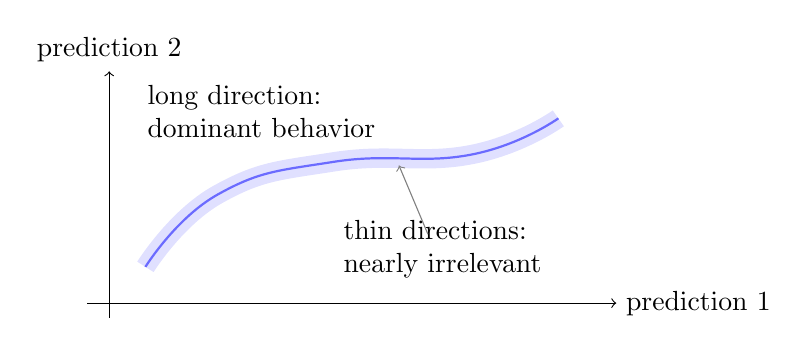
\begin{tikzpicture}[scale=0.92]
  \draw[->] (-0.3,0) -- (7,0) node[right] {prediction 1};
  \draw[->] (0,-0.2) -- (0,3.2) node[above] {prediction 2};
  \draw[thick,blue!70] plot[smooth,tension=0.8] coordinates {(0.5,0.5) (1.5,1.5) (3.1,1.95) (5.0,2.05) (6.2,2.55)};
  \draw[blue!35,line width=7pt,opacity=0.35] plot[smooth,tension=0.8] coordinates {(0.5,0.5) (1.5,1.5) (3.1,1.95) (5.0,2.05) (6.2,2.55)};
  \node[align=left] at (4.6,0.75) {thin directions:\\nearly irrelevant};
  \draw[->,gray] (4.4,0.95) -- (4.0,1.9);
  \node[align=left] at (2.1,2.65) {long direction:\\dominant behavior};
\end{tikzpicture}
\end{center}

\subsection{Boundaries as approximations}

If a manifold is thin, its boundary may be a good lower-dimensional approximation.  Algebraically, boundaries often correspond to limits:
\[
  k\to 0,\qquad
  k\to\infty,\qquad
  \frac{k_1}{k_2}\to K,\qquad
  \tau_{\mathrm{fast}}\to 0.
\]
Scientifically, these limits are familiar: irreversible reactions, equilibrium approximations, quasi-steady state approximations, continuum limits, thermodynamic limits, and fast-mode elimination.  So a boundary is not a mathematical accident.  It is often an old modeling approximation rediscovered by asking what the data cannot distinguish.

\section{MBAM: walking from weak direction to simpler mechanism}

\subsection{The algorithm}

The Manifold Boundary Approximation Method can be summarized as:
\begin{enumerate}[leftmargin=2em]
  \item Choose the quantities of interest \(\qoi\).
  \item Compute the Fisher information \(\fim(\param)\).
  \item Find the least informative eigenvector.
  \item Follow a geodesic in that direction until the model manifold reaches a boundary.
  \item Identify the limiting approximation in the original equations.
  \item Replace the full model by the boundary model and refit.
  \item Repeat until the model is simple enough for the scientific question.
\end{enumerate}

The important point is that MBAM removes parameter combinations, not merely named parameters.  It begins with the same local matrix story as SVD, but it refuses to stop at a local vector; it walks until the equations reveal a limit.

\subsection{Geodesic equation}

On a manifold with metric \(g_{ij}\), a geodesic satisfies
\[
  \ddot{\theta}^i+\Gamma^i_{jk}\dot{\theta}^j\dot{\theta}^k=0.
\]
Here \(g_{ij}\) is the Fisher metric.  The geodesic starts in the least sensitive direction.  As it approaches a boundary, the limiting form often becomes interpretable: one rate goes to zero, two rates go to infinity with fixed ratio, a fast variable equilibrates, or two modes merge.

\begin{remark}
  The geodesic is a numerical flashlight.  It does not itself explain the biology; it shows where to look in the equations for the simplifying limit.
\end{remark}

\subsection{Why this is not black-box reduction}

Many reduction methods produce a smaller system that predicts well but is hard to interpret.  MBAM tries to preserve mechanistic meaning by taking limits inside the original model.  The reduced model remains expressed in terms of original mechanisms or combinations of them.

That is why MBAM is attractive for QSP: a regulatory or pharmacological model must not only predict.  It must explain what biological simplification has been made.

\section{Boundary examples: the abstractions become mechanisms}

\subsection{Sum of exponentials}

Consider
\[
  y(t;\param)
  =
  \sum_{j=1}^N A_j e^{-\lambda_j t}.
\]
If one rate is much faster than all observed sampling times,
\[
  \lambda_j\to\infty,
  \qquad
  A_j e^{-\lambda_j t}\approx 0
  \quad(t>0).
\]
If one rate is much slower than the experiment,
\[
  \lambda_j\to 0,
  \qquad
  A_j e^{-\lambda_j t}\approx A_j.
\]
If two rates merge,
\[
  A_1e^{-\lambda t}+A_2e^{-\lambda t}
  =
  (A_1+A_2)e^{-\lambda t}.
\]
These are manifold boundaries with simple physical meaning: unobserved fast decay, constant slow background, and merged modes.  Notice the full chain: LTI gives exponentials, SVD notices indistinguishable combinations, the manifold picture calls them boundaries, and MBAM turns the boundary into a reduced model.

\subsection{Michaelis--Menten}

The enzyme scheme
\[
  E+S
  \xrightleftharpoons[k_r]{k_f}
  C
  \xrightarrow{k_c}
  E+P
\]
has a boundary where \(k_f,k_r\to\infty\) with \(K_d=k_r/k_f\) fixed.  The fast binding step equilibrates:
\[
  C\approx \frac{E S}{K_d}.
\]
Using conservation of enzyme, the product rate becomes
\[
  \ddt P
  =
  \frac{k_c E_0 S}{K_d+S}.
\]
MBAM recovers this familiar approximation geometrically: the data cannot distinguish the two fast rates separately, only their effective combination.

\subsection{An LTI reduction}

Suppose an LTI model contains a fast pole \(-\beta\) and a slow pole \(-\alpha\), with \(\beta\gg\alpha\).  If the query ignores very early transients, then the fast mode is a thin direction in prediction space.  A boundary approximation removes it:
\[
  e^{-\beta t}\to 0
  \quad\text{on the query window.}
\]
The reduced model is not universally equivalent to the full model.  It is equivalent relative to the quantities of interest.  This phrase, relative to the quantities of interest, is the heartbeat of MBAM.

\section{QSP and CRISP: the query closes the loop}

\subsection{QSP as query-driven modeling}

QSP models become large because they collect plausible mechanisms.  But a decision rarely needs every mechanism at full resolution.  A toxicology query, a dose-selection query, and a target-discovery query may require different reduced models.

Let training data be \(\data\) and future quantities of interest be \(\qoi\).  The modeling problem is not merely
\[
  \text{fit }\data.
\]
It is
\[
  \text{extract from }\data
  \text{ the information needed for }\qoi.
\]
This is the conceptual bridge from information geometry to QSP workflow.  A model is not reduced in the abstract; it is reduced for a decision.

\subsection{CRISP language}

The CRISP idea can be read as:
\[
  \begin{array}{c}
    \text{comprehensive model}\\
    \downarrow\\
    \text{calibrated model}\\
    \downarrow\\
    \text{query-specific active manifold}\\
    \downarrow\\
    \text{fit-for-purpose reduced model}
  \end{array}
\]
The reduction is contextual.  It is not saying the removed mechanism is false.  It is saying the mechanism is irrelevant to the specified prediction at the specified precision.

\subsection{Mechanistic control knobs}

The best reduced model does more than save computation.  It identifies control knobs:
\[
  \phi_1(\param),\ldots,\phi_k(\param)
\]
such that the quantities of interest depend mainly on \(\phi\), not on all microscopic parameters.  In systems biology, these combinations may correspond to time-scale ratios, saturation constants, feedback strengths, or pathway capacities.  This is the end of the chain that began with a Jacobian: a singular direction becomes a mechanistic control knob.

\section{Plate notation for QSP: the probabilistic shell around mechanism}

\subsection{Why a QSP diagram is not enough}

A traditional QSP diagram is excellent at showing mechanistic flow: ligand activates receptor, receptor changes signaling, signaling changes biomarker, biomarker affects phenotype.  But it often hides the probabilistic architecture:
\begin{itemize}[leftmargin=2em]
  \item Which quantities are fixed design choices?
  \item Which biological states are latent and inferred?
  \item Which parameters vary between individuals?
  \item Which measurements are noisy observations of hidden states?
  \item Where do covariates, omics features, or AI-derived latent features enter?
\end{itemize}
Plate notation answers a different question from a pathway diagram.  A pathway diagram says what interacts mechanistically.  A plate diagram says what is random, what is observed, what is repeated, and what conditions what.

\subsection{A minimal QSP plate}

For a QSP model with \(N\) individuals and \(T_i\) observation times, a probabilistic shell can be drawn as:

\begin{center}
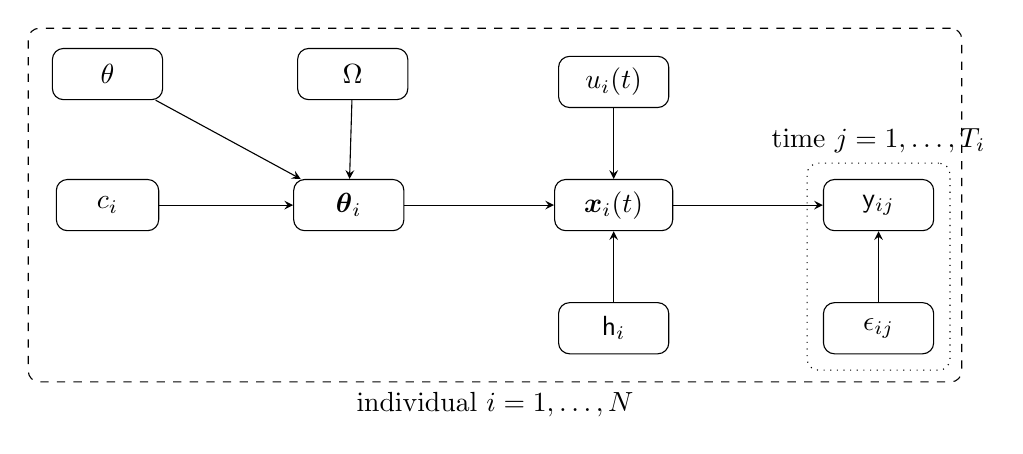
\begin{tikzpicture}[>=stealth, node distance=1.35cm, every node/.style={align=center}]
  \node[draw, rounded corners, minimum width=1.4cm, minimum height=0.65cm] (theta) {\(\theta\)};
  \node[draw, rounded corners, right=1.7cm of theta, minimum width=1.4cm, minimum height=0.65cm] (omega) {\(\Omega\)};
  \node[draw, rounded corners, below=1.0cm of theta, minimum width=1.3cm, minimum height=0.65cm] (c) {\(c_i\)};
  \node[draw, rounded corners, right=1.7cm of c, minimum width=1.4cm, minimum height=0.65cm] (psi) {\(\rtheta_i\)};
  \node[draw, rounded corners, right=1.9cm of psi, minimum width=1.5cm, minimum height=0.65cm] (x) {\(\rx_i(t)\)};
  \node[draw, rounded corners, right=1.9cm of x, minimum width=1.4cm, minimum height=0.65cm] (y) {\(\rv{y}_{ij}\)};
  \node[draw, rounded corners, above=0.9cm of x, minimum width=1.4cm, minimum height=0.65cm] (u) {\(u_i(t)\)};
  \node[draw, rounded corners, below=0.9cm of x, minimum width=1.4cm, minimum height=0.65cm] (h) {\(\rv{h}_i\)};
  \node[draw, rounded corners, below=0.9cm of y, minimum width=1.4cm, minimum height=0.65cm] (eps) {\(\epsilon_{ij}\)};

  \draw[->] (theta) -- (psi);
  \draw[->] (omega) -- (psi);
  \draw[->] (c) -- (psi);
  \draw[->] (psi) -- (x);
  \draw[->] (u) -- (x);
  \draw[->] (h) -- (x);
  \draw[->] (x) -- (y);
  \draw[->] (eps) -- (y);

  \node[draw, dashed, rounded corners, fit=(c)(psi)(x)(y)(u)(h)(eps), inner sep=0.35cm, label=below:{individual \(i=1,\ldots,N\)}] {};
  \node[draw, dotted, rounded corners, fit=(y)(eps), inner sep=0.20cm, label=above:{time \(j=1,\ldots,T_i\)}] {};
\end{tikzpicture}
\captionof{figure}{A QSP plate separates the mechanistic state equation from the probabilistic hierarchy.  The mechanistic ODE lives inside \(\rx_i(t)\); the plate tells us how population parameters, individual variation, covariates, latent features, design, and measurement error generate observed biomarkers.}
\end{center}

The corresponding verbal model is:
\[
  \rtheta_i\sim p_\theta(\theta_i\given c_i,\Omega),
  \qquad
  \frac{\dd \rx_i(t)}{\dd t}=f(\rx_i(t),\rtheta_i,u_i(t),\rv{h}_i),
  \qquad
  \rv{y}_{ij}\sim p(y_{ij}\given \rx_i(t_{ij}),\epsilon_{ij}).
\]
The ODE gives causality inside a subject.  The plate gives replication, uncertainty, and observation.

\subsection{What the plate buys us in toxicology}

The GRC toxicology draft's core idea is that plate notation is a visual grammar for mechanistic models with uncertainty.  In QSP toxicology, this is especially helpful because the model often combines:
\begin{itemize}[leftmargin=2em]
  \item hierarchical variability across donors, cell lines, animals, or patients;
  \item latent biological states such as injury stage, pathway activation, or target-site exposure;
  \item noisy biomarkers, omics measurements, and histopathology endpoints;
  \item AI/ML-derived features that summarize images, transcripts, or high-dimensional assays;
  \item regulatory decisions that require reproducible model structure, not only successful prediction.
\end{itemize}
The plate does not replace the QSP mechanism.  It wraps the mechanism in a probabilistic contract.  Once the contract is visible, different teams can ask precise questions: which latent states are inferred, which variables are measured, which dependencies are assumed, and which modules can be recombined without changing the meaning of the model.

\begin{remark}
  This is also where Bayesian modeling and MBAM meet.  Plate notation says which uncertainty structure surrounds the QSP map; MBAM asks which mechanistic directions inside that map are distinguishable for the query.  One clarifies the probabilistic shell, the other clarifies the mechanistic core.
\end{remark}

\section{Detailed worked notebook: the same spine in slow motion}

The following workbook is not a second, unrelated set of chapters.  It repeats the same spine at lower altitude.  The first group builds the linear and statistical geometry.  The second group shows how ODE/LTI systems create the relevant sensitivities and time scales.  The third group turns those sensitivities into Fisher geometry and model manifolds.  The final group shows how boundaries become MBAM and CRISP reductions.  Read it as a spiral: each example returns to
\[
  \begin{array}{c}
    \param\longmapsto\vect{y}(\param)\longmapsto\jac(\param)\\
    \downarrow\\
    \fim(\param)\longmapsto\text{boundary}
  \end{array}
\]

\noindent
The worked notebook repeats the main spine at slower speed.  The first pass is purely linear: covariance gives shape, projection gives fitting, derivatives give the local map, and the SVD tells us which combinations are visible.

\subsection{Covariance as geometry}

\subsubsection*{Why covariance is a matrix}

For a random vector \(\rv{x}\in\R^n\), covariance is
\[
  \Cov(\rv{x})
  =
  \E\left[
    (\rv{x}-\mu)(\rv{x}-\mu)^{\transpose}
  \right].
\]
The diagonal entries are variances.  The off-diagonal entries are co-movements.  But the geometric meaning is stronger: covariance defines the shape of uncertainty.  If
\[
  \rv{x}\sim\mathcal{N}(\mu,\Sigma),
\]
then contours of equal density are ellipsoids:
\[
  (\vect{x}-\mu)^{\transpose}\Sigma^{-1}(\vect{x}-\mu)=c.
\]
Large eigenvalues of \(\Sigma\) are broad uncertainty directions.  Small eigenvalues are tightly known directions.

\subsubsection*{The duality with information}

In a regular Gaussian approximation, the parameter covariance is approximately the inverse Fisher information:
\[
  \Cov(\widehat{\param})
  \approx
  \fim(\widehat{\param})^{-1}.
\]
So the eigenvectors of \(\Sigma\) and \(\fim\) point in the same directions, but their eigenvalues invert.  A large covariance direction is a small information direction.  This is one of the cleanest bridges between statistics and numerical linear algebra.

\subsection{Projection and least squares}

\subsubsection*{The nearest point problem}

Given \(\mat{A}\in\R^{m\times n}\) and \(\vect{b}\in\R^m\), least squares asks for
\[
  \widehat{\vect{x}}
  =
  \argmin_{\vect{x}}
  \norm{\mat{A}\vect{x}-\vect{b}}_2^2.
\]
If \(\mat{A}\) has full column rank, the solution satisfies
\[
  \mat{A}^{\transpose}\mat{A}\widehat{\vect{x}}
  =
  \mat{A}^{\transpose}\vect{b}.
\]
This is not magic.  At the closest point, the residual must be orthogonal to every column direction:
\[
  \mat{A}^{\transpose}(\mat{A}\widehat{\vect{x}}-\vect{b})=0.
\]

\subsubsection*{Weighted projection}

If measurements have covariance \(\Sigma\), the geometry changes:
\[
  \widehat{\vect{x}}
  =
  \argmin_{\vect{x}}
  (\mat{A}\vect{x}-\vect{b})^{\transpose}
  \Sigma^{-1}
  (\mat{A}\vect{x}-\vect{b}).
\]
The normal equations become
\[
  \mat{A}^{\transpose}\Sigma^{-1}\mat{A}\widehat{\vect{x}}
  =
  \mat{A}^{\transpose}\Sigma^{-1}\vect{b}.
\]
Whitening with \(\Sigma^{-1/2}\) turns the weighted problem into an ordinary Euclidean projection.  This is exactly what scaled residuals do in model fitting.

\subsection{Matrix derivatives}

\subsubsection*{Differentials first}

Matrix calculus is least confusing when written with differentials.  If
\[
  f(\vect{x})=\frac{1}{2}\vect{x}^{\transpose}\mat{A}\vect{x},
\]
then
\[
  \dd f
  =
  \frac{1}{2}\dd\vect{x}^{\transpose}\mat{A}\vect{x}
  +
  \frac{1}{2}\vect{x}^{\transpose}\mat{A}\dd\vect{x}.
\]
If \(\mat{A}\) is symmetric,
\[
  \dd f=(\mat{A}\vect{x})^{\transpose}\dd\vect{x},
  \qquad
  \nabla f=\mat{A}\vect{x}.
\]
The Hessian is \(\mat{A}\).

\subsubsection*{Trace trick}

The trace identity
\[
  \tr(\mat{A}\mat{B})=\tr(\mat{B}\mat{A})
\]
lets us move differentials to the end.  For
\[
  f(\mat{X})=\frac{1}{2}\norm{\mat{A}\mat{X}-\mat{B}}_F^2,
\]
we have
\[
  \dd f
  =
  \tr\left[
    (\mat{A}\mat{X}-\mat{B})^{\transpose}\mat{A}\,\dd\mat{X}
  \right],
\]
so
\[
  \nabla_{\mat{X}} f
  =
  \mat{A}^{\transpose}(\mat{A}\mat{X}-\mat{B}).
\]
This is the same normal-equation geometry in matrix form.

\subsection{Whitening and likelihood}

\subsubsection*{Gaussian residuals}

Suppose
\[
  \vect{d}
  =
  \vect{y}(\param)+\rv{\epsilon},
  \qquad
  \rv{\epsilon}\sim\mathcal{N}(0,\Sigma).
\]
The negative log likelihood, up to constants, is
\[
  \loss(\param)
  =
  \frac{1}{2}
  (\vect{d}-\vect{y}(\param))^{\transpose}
  \Sigma^{-1}
  (\vect{d}-\vect{y}(\param)).
\]
Let
\[
  \widetilde{\vect{r}}(\param)
  =
  \Sigma^{-1/2}
  (\vect{y}(\param)-\vect{d}).
\]
Then
\[
  \loss(\param)=\frac{1}{2}\norm{\widetilde{\vect{r}}(\param)}^2.
\]
Likelihood turns into Euclidean geometry after whitening.

\subsubsection*{Scaled sensitivity}

The whitened Jacobian is
\[
  \widetilde{\jac}
  =
  \Sigma^{-1/2}
  \pd{\vect{y}}{\param}.
\]
The Fisher information is
\[
  \fim=\widetilde{\jac}^{\transpose}\widetilde{\jac}.
\]
Thus experimental uncertainty is not an afterthought.  It changes the metric on parameter space and therefore changes which directions are stiff or sloppy.

\subsection{Identifiable combinations by SVD}

\subsubsection*{Linearized model}

Linearize a nonlinear prediction around \(\param_0\):
\[
  \delta\vect{y}
  =
  \jac\delta\param.
\]
Take the SVD
\[
  \jac=\mat{U}\Sigma\mat{V}^{\transpose}.
\]
Then
\[
  \delta\vect{y}
  =
  \sum_j
  \sigma_j
  \vect{u}_j
  (\vect{v}_j^{\transpose}\delta\param).
\]
The scalar
\[
  \phi_j=\vect{v}_j^{\transpose}\param
\]
is a locally identifiable combination if \(\sigma_j\) is large.

\subsubsection*{A practical interpretation}

If a paper reports huge uncertainty in individual rate constants but stable predictions, do not immediately call the model bad.  Ask whether the predictions depend on a few combinations.  The raw parameters may be poorly identified while the scientifically relevant combinations are sharply constrained.

\noindent
The second pass puts the same linear ideas inside time.  An ODE is not a different subject here; it is the machine that produces \(\vect{y}(\param)\), and its sensitivities are the Jacobian columns we have already learned to read.

\subsection{Exponential decay}

\subsubsection*{One parameter}

Consider
\[
  y(t;k)=A e^{-kt}.
\]
The sensitivity to \(k\) is
\[
  \pd{y}{k}
  =
  -tA e^{-kt}.
\]
Early time points have little sensitivity to \(k\), because \(t\) is small.  Late time points may also have little sensitivity if \(e^{-kt}\) is already near zero.  The most informative time scale is around \(t\sim 1/k\).

\subsubsection*{Two parameters}

Now let
\[
  y(t;A,k)=A e^{-kt}.
\]
The Jacobian row at time \(t_m\) is
\[
  \begin{bmatrix}
    e^{-kt_m} & -t_m A e^{-kt_m}
  \end{bmatrix}.
\]
If all observations are very early, then
\[
  e^{-kt}\approx 1-kt,
  \qquad
  A e^{-kt}\approx A-Akt.
\]
The data mainly see \(A\) and \(Ak\), not \(A\) and \(k\) independently.  This is a baby version of identifiable combinations.

\subsection{Sums of exponentials}

\subsubsection*{Why they become sloppy}

For
\[
  y(t)=\sum_{j=1}^N A_j e^{-\lambda_j t},
\]
nearby rates can compensate:
\[
  A_1e^{-\lambda_1 t}+A_2e^{-\lambda_2 t}
  \approx
  (A_1+A_2)e^{-\bar{\lambda}t}
\]
over a finite time window if \(\lambda_1\) and \(\lambda_2\) are close.  Very fast rates disappear after the early transient.  Very slow rates look nearly constant.  These are not numerical coincidences; they are model manifold boundaries.

\subsubsection*{Connection to LTI}

Every stable finite-dimensional LTI system has impulse responses made from exponentials, possibly multiplied by polynomials for repeated poles.  Therefore the exponential-sum example is not a toy disconnected from systems theory.  It is the scalar shadow of modal decomposition.

\subsection{Sensitivity ODE}

\subsubsection*{Derivation}

Let
\[
  \dot{\vect{x}}=\vect{f}(\vect{x},\param),
  \qquad
  \vect{x}(0)=\vect{x}_0(\param).
\]
Set
\[
  \mat{S}(t)=\pd{\vect{x}(t)}{\param}
  \in\R^{n\times p}.
\]
Differentiate both sides with respect to \(\param\):
\[
  \dot{\mat{S}}
  =
  \pd{\vect{f}}{\vect{x}}\mat{S}
  +
  \pd{\vect{f}}{\param},
  \qquad
  \mat{S}(0)=\pd{\vect{x}_0}{\param}.
\]
This sensitivity system is linear in \(\mat{S}\), even when the original ODE is nonlinear.

\subsubsection*{Why finite differences can mislead}

Finite differences approximate
\[
  \pd{\vect{y}}{\theta_i}
  \approx
  \frac{\vect{y}(\param+h\vect{e}_i)-\vect{y}(\param)}{h}.
\]
If \(h\) is too large, the approximation is nonlinear.  If \(h\) is too small, floating-point cancellation dominates.  Sensitivity equations avoid many of these problems, which is why MBAM implementations often prefer them for ODE models.

\subsection{Two-compartment dynamics}

\subsubsection*{A minimal PK-like LTI system}

Consider
\[
  \ddt
  \begin{bmatrix}
    C_1\\ C_2
  \end{bmatrix}
  =
  \begin{bmatrix}
    -(k_{10}+k_{12}) & k_{21}\\
    k_{12} & -k_{21}
  \end{bmatrix}
  \begin{bmatrix}
    C_1\\ C_2
  \end{bmatrix}.
\]
The eigenvalues of the system matrix produce two exponential phases.  If one phase is much faster than the sampling resolution, it may be practically invisible.

\subsubsection*{Boundary interpretation}

A fast exchange limit such as
\[
  k_{12},k_{21}\to\infty,
  \qquad
  \frac{k_{12}}{k_{21}}\to \rho
\]
can collapse two compartments into a quasi-equilibrated effective compartment.  The surviving parameter is not \(k_{12}\) or \(k_{21}\) alone, but a ratio or capacity-like combination.  This is exactly the kind of limit MBAM is designed to reveal.

\subsection{Spring--mass--damper}

\subsubsection*{Second-order equation}

The classical LTI example is
\[
  m\ddot{x}+b\dot{x}+kx=f(t).
\]
The transfer function from force to displacement is
\[
  H(s)=\frac{1}{ms^2+bs+k}.
\]
The poles solve
\[
  ms^2+bs+k=0.
\]
They encode damping, oscillation, and stability.

\subsubsection*{Nondimensional form}

Define
\[
  \omega_n=\sqrt{\frac{k}{m}},
  \qquad
  \zeta=\frac{b}{2\sqrt{mk}}.
\]
Then
\[
  \ddot{x}+2\zeta\omega_n\dot{x}+\omega_n^2x=\frac{1}{m}f(t).
\]
The three physical parameters \(m,b,k\) become combinations \(\omega_n,\zeta,1/m\).  Often these combinations are more interpretable than the raw parameters.

\subsection{Convolution}

\subsubsection*{Impulse response}

If \(h(t)\) is the impulse response, any input \(u(t)\) produces
\[
  y(t)=\int_0^t h(t-\tau)u(\tau)\,\dd\tau.
\]
Convolution says that the system remembers past input through a kernel.  A fast kernel has short memory; a slow kernel has long memory.

\subsubsection*{Relevance of memory}

For a QSP model, deciding whether a subsystem can be reduced often means asking: does its memory kernel matter on the query time scale?  If not, it may be replaced by an algebraic relation, an effective delay, or a lower-order state.

\subsection{Stiffness}

\subsubsection*{Multiple time scales}

An ODE is stiff when stable fast modes force tiny numerical steps even though the scientific behavior of interest evolves slowly.  A simple linear example is
\[
  \dot{x}_1=-x_1,
  \qquad
  \dot{x}_2=-1000x_2.
\]
The second state decays rapidly, but explicit numerical methods may still be constrained by it.

\subsubsection*{Model reduction view}

Stiffness and sloppiness are not the same, but they often meet.  A fast stable mode may be numerically troublesome and prediction-irrelevant after a short transient.  A boundary approximation can remove it if the quantities of interest do not ask about that transient.

\noindent
The third pass asks whether our computations are honest enough to support scientific interpretation.  Conditioning, regularization, and stable factorization are not numerical footnotes; they decide whether a small singular value is a property of the model or an artifact of the calculation.

\subsection{Finite precision}

\subsubsection*{Roundoff as perturbation}

Floating-point arithmetic replaces exact operations by perturbed operations.  A computed solution often solves a nearby problem:
\[
  (\mat{A}+\delta\mat{A})\widehat{\vect{x}}=\vect{b}+\delta\vect{b}.
\]
Backward error analysis asks whether the nearby problem is close enough to the original one.

\subsubsection*{Scientific analogy}

Model reduction has a similar flavor.  A reduced model is acceptable if it solves a nearby prediction problem at the precision required by the scientific question.  The question is not whether the reduced model is literally identical.  It is whether the discrepancy is smaller than the relevant tolerance.

\subsection{Regularization}

\subsubsection*{Ridge}

Ridge regression solves
\[
  \widehat{\vect{x}}
  =
  \argmin_{\vect{x}}
  \norm{\mat{A}\vect{x}-\vect{b}}^2
  +
  \lambda\norm{\vect{x}}^2.
\]
The solution is
\[
  \widehat{\vect{x}}
  =
  (\mat{A}^{\transpose}\mat{A}+\lambda\eye)^{-1}
  \mat{A}^{\transpose}\vect{b}.
\]
It suppresses directions with small singular values.

\subsubsection*{Relation to Bayesian priors}

The penalty \(\lambda\norm{\vect{x}}^2\) is equivalent to a Gaussian prior on \(\vect{x}\).  In mechanistic modeling, regularization can stabilize fitting, but it does not by itself explain which mechanisms are irrelevant.  MBAM aims for an explanatory reduction rather than only a stabilized inverse problem.

\subsection{QR versus normal equations}

\subsubsection*{Squaring the condition number}

Solving least squares through
\[
  \mat{A}^{\transpose}\mat{A}\vect{x}
  =
  \mat{A}^{\transpose}\vect{b}
\]
can be numerically dangerous because
\[
  \kappa(\mat{A}^{\transpose}\mat{A})=\kappa(\mat{A})^2.
\]
QR and SVD avoid this squaring.

\subsubsection*{Model-fitting moral}

If a fitting problem is already ill-conditioned, careless numerical formulation can make it worse.  Before interpreting parameter uncertainty scientifically, we need to know whether the uncertainty comes from the model/data geometry or from unstable computation.

\noindent
The fourth pass changes the distance measure.  Least squares measured Euclidean residuals; inference measures distinguishability between probability laws.  Fisher information is the bridge that lets the same Jacobian language survive this change.

\subsection{KL local expansion}

\subsubsection*{One-dimensional sketch}

Let \(p(x\mid\theta)\) be smooth.  The score is
\[
  s_\theta(x)=\pd{}{\theta}\log p(x\mid\theta).
\]
Under regularity conditions,
\[
  \E_\theta[s_\theta(\rv{x})]=0.
\]
The Fisher information is
\[
  I(\theta)=\E_\theta[s_\theta(\rv{x})^2].
\]
Then for small \(\delta\),
\[
  \KL(p_\theta\|p_{\theta+\delta})
  =
  \frac{1}{2}I(\theta)\delta^2+o(\delta^2).
\]

\subsubsection*{Why the first-order term vanishes}

The first-order term vanishes because probabilities must still integrate to one:
\[
  \int p(x\mid\theta)\,\dd x=1
  \quad\Rightarrow\quad
  \int \pd{p(x\mid\theta)}{\theta}\,\dd x=0.
\]
This is the probabilistic reason Fisher information is second-order geometry.

\subsection{Information projection}

\subsubsection*{Projection between distributions}

Information projection asks for the member of a family closest in KL divergence:
\[
  Q^\star
  =
  \argmin_{Q\in\mathcal{F}}
  \KL(P\|Q).
\]
This is not Euclidean projection, but it plays a similar role in statistical geometry.

\subsubsection*{Model reduction reading}

When a reduced model family is used to approximate a full model, we can think of the reduced family as a lower-dimensional surface.  The best reduced model is the projection of the full model's behavior onto that surface, according to the distinguishability relevant to the query.

\subsection{Model manifold for line fitting}

\subsubsection*{A simple surface}

Let
\[
  y_i(a,b)=a+bt_i
\]
for fixed time points \(t_i\).  The prediction vector is
\[
  \vect{y}(a,b)=a\vect{1}+b\vect{t}.
\]
The model manifold is a plane in \(\R^M\).  The Jacobian is constant:
\[
  \jac=
  \begin{bmatrix}
    1 & t_1\\
    \vdots & \vdots\\
    1 & t_M
  \end{bmatrix}.
\]

\subsubsection*{Why nonlinear models are different}

For nonlinear models, the tangent plane changes with \(\param\).  Small eigenvectors of the Fisher information may rotate as we move.  This is why MBAM follows a geodesic instead of simply deleting the smallest local singular vector at the starting point.

\noindent
The final pass stops being merely local.  A sloppy direction at one point becomes useful only when we follow it until the equations reveal a boundary, a limit, or an approximation we can name.

\subsection{Geodesic boundaries}

\subsubsection*{Local direction, nonlocal limit}

The least sensitive eigenvector is local:
\[
  \fim(\param_0)\vect{v}_{\min}
  =
  \lambda_{\min}\vect{v}_{\min}.
\]
Following the geodesic reveals how that direction evolves.  Near a boundary, the direction often simplifies and points toward a recognizable parameter limit.

\subsubsection*{The interpretive step}

The numerical geodesic might say:
\[
  k_1\to\infty,
  \qquad
  k_2\to\infty,
  \qquad
  \frac{k_2}{k_1}\to K.
\]
The modeler must then inspect the equations and take the limit carefully.  The resulting reduced model is the scientific product.

\subsection{Boundary taxonomy}

\subsubsection*{Common limits}

MBAM often finds limits such as:
\[
  k\to 0,\quad
  k\to\infty,\quad
  \frac{k_1}{k_2}\to K,\quad
  x_{\mathrm{fast}}\to x_{\mathrm{eq}},\quad
  N\to\infty,\quad
  \Delta x\to 0.
\]
These correspond to irreversibility, fast equilibration, quasi-steady state, thermodynamic limit, and continuum limit.

\subsubsection*{Why limits preserve meaning}

Deleting a variable by numerical black-box projection may preserve output but hide mechanism.  Taking a limit inside the original equations shows what physical or biological assumption is being made.

\subsection{MBAM and Michaelis--Menten carefully}

\subsubsection*{Mass action}

For
\[
  E+S
  \xrightleftharpoons[k_r]{k_f}
  C
  \xrightarrow{k_c}
  E+P,
\]
mass action gives
\[
  \dot{C}=k_fES-(k_r+k_c)C.
\]
If binding/unbinding is fast relative to catalysis, then \(k_f,k_r\to\infty\) with \(K_d=k_r/k_f\) fixed.  The fast equation imposes
\[
  k_fES-k_rC\approx 0
  \quad\Rightarrow\quad
  C\approx \frac{ES}{K_d}.
\]

\subsubsection*{Conservation}

With \(E_0=E+C\),
\[
  C
  =
  \frac{(E_0-C)S}{K_d}
  \quad\Rightarrow\quad
  C(K_d+S)=E_0S.
\]
Thus
\[
  C=\frac{E_0S}{K_d+S},
  \qquad
  \dot{P}=k_cC
  =
  \frac{k_cE_0S}{K_d+S}.
\]
The reduced model keeps the combination \(K_d=k_r/k_f\), not the two fast rates separately.

\noindent
The last two examples close the loop back to QSP.  Once the reduced mechanism exists, we still have to ask which prediction it was reduced for, and whether the decision query really ignores what we removed.

\subsection{Active manifold}

\subsubsection*{Training data versus query}

Let \(\data\) be calibration data and \(\qoi\) future predictions.  A parameter direction can be irrelevant to \(\qoi\) even if it affects unobserved internal variables.  Conversely, a direction can fit \(\data\) weakly but matter greatly for a future intervention.

This is why reduction should be query-specific:
\[
  \fim_{\qoi}
  =
  \jac_{\qoi}^{\transpose}\jac_{\qoi}.
\]

\subsubsection*{The active subspace}

The stiff eigendirections of \(\fim_{\qoi}\) span an active local subspace.  MBAM asks whether the inactive directions can be pushed to boundaries and removed while retaining the active behavior.  The result is not merely lower dimension; it is a simpler mechanistic explanation for the query.

\subsection{CRISP for QSP}

\subsubsection*{A workflow}

For a QSP project, a CRISP-like workflow reads:
\begin{enumerate}[leftmargin=2em]
  \item Build a literature-derived mechanistic model.
  \item Calibrate enough to make the model behave plausibly.
  \item Define the query: virtual population, target discovery, toxicology, dose selection, or biomarker prediction.
  \item Compute sensitivities of the query.
  \item Use information geometry to identify irrelevant combinations.
  \item Reduce by MBAM boundaries.
  \item Refit and validate the reduced model for the query.
\end{enumerate}

\subsubsection*{Regulatory style interpretation}

For model-informed decisions, a reduced QSP model should answer:
\[
  \begin{array}{c}
    \text{What was removed?}\\
    \text{Why is it irrelevant?}\\
    \text{For which prediction is it irrelevant?}
  \end{array}
\]
This is the standard we should use in future pharmacology notes.

\subsection{The full conceptual chain}

\subsubsection*{From matrix to manifold}

The chain is:
\[
  \mat{A}
  \quad\leadsto\quad
  \jac
  \quad\leadsto\quad
  \jac^{\transpose}\jac
  \quad\leadsto\quad
  \fim
  \quad\leadsto\quad
  \text{metric}
  \quad\leadsto\quad
  \text{model manifold}.
\]
Each arrow changes vocabulary but preserves a central idea: how does a small movement in one space become a movement in another space?

\subsubsection*{From ODE to MBAM}

The dynamic chain is:
\[
  \begin{array}{c}
    \dot{\vect{x}}=\vect{f}(\vect{x},\param)
    \quad\leadsto\quad
    \vect{y}(\param)
    \quad\leadsto\quad
    \pd{\vect{y}}{\param}\\
    \downarrow\\
    \text{least visible parameter direction}
    \quad\leadsto\quad
    \text{boundary limit}
  \end{array}
\]
That is the mathematical skeleton beneath many successful approximations in biology and pharmacology.


\section{A self-study route}

\subsection{The order I would read}

I would not start with MBAM directly.  I would read in this order:
\begin{enumerate}[leftmargin=2em]
  \item 6.S087 probability and matrix tricks: random variables, covariance, gradients, Jacobians.
  \item Matrix Cookbook: identities as a reference, not as a book to memorize.
  \item 18.03: ODE modeling, units, linearization, qualitative behavior.
  \item 18.031: LTI systems, convolution, transfer functions, poles.
  \item 18.335: conditioning, residual/error distinction, QR/SVD, iterative methods.
  \item 6.441: divergence, local Fisher geometry, information projection.
  \item 6.435: Bayesian workflow, plate notation, approximate inference, and model criticism.
  \item MBAM papers: model manifold, geodesics, boundary limits.
  \item QSP CRISP paper: how these ideas become a workflow for pharmacological models.
\end{enumerate}

\subsection{A reading checklist for any model}

When reading a QSP or systems biology model, ask:
\begin{enumerate}[leftmargin=2em]
  \item What are the states \(\vect{x}\)?
  \item What are the parameters \(\param\)?
  \item What are the quantities of interest \(\qoi\)?
  \item What is the prediction map \(\param\mapsto\vect{y}(\param)\)?
  \item What is observed, what is latent, and what plate structure repeats across subjects, times, tissues, or assays?
  \item How is \(\jac=\partial\vect{y}/\partial\param\) computed?
  \item What are the large and small singular directions?
  \item Which small directions correspond to interpretable limits?
  \item Does the reduced model preserve the prediction task, or only the training data?
  \item What mechanistic combinations survive as control knobs?
\end{enumerate}

\section{Connection back to pharmacology}

\subsection{Why this belongs next to PK/PD}

Population PK taught us that individual parameters are latent and inferred through a hierarchical model.  MBAM teaches a complementary lesson: mechanistic parameters may be too detailed for the prediction task, and the meaningful objects may be combinations living on a lower-dimensional manifold.

In PK/PD terms:
\[
  \begin{array}{c}
    \text{rich mechanism}\\
    \downarrow\\
    \text{prediction map}\\
    \downarrow\\
    \text{active combinations}\\
    \downarrow\\
    \text{decision-ready reduced model}
  \end{array}
\]
This is exactly what we want when moving from detailed QSP to dosing, target discovery, biomarker selection, or trial design.

\subsection{The one-sentence memory hook}

\begin{quote}
  MBAM is numerical linear algebra plus information geometry applied to mechanistic dynamical models: it follows the least identifiable direction until the equations reveal a scientifically meaningful limiting approximation.
\end{quote}

\subsection{Working conclusion}

Linear algebra teaches how maps stretch directions.  ODE teaches how biological mechanisms generate maps over time.  LTI theory teaches modes, poles, convolution, and time scales.  Numerical analysis teaches which computations and inverse problems are trustworthy.  Information geometry teaches that distinguishability is a metric.  MBAM combines these lessons into a practical question:
\begin{quote}
  Which parts of this mechanistic model are truly needed for this prediction?
\end{quote}

That question is small enough to compute and large enough to guide QSP.

\end{document}
